%%%%%%%%%%%%%%%%%%%%%%%%%%%%%%%%%%%%%%%%%%%%%%%%%%%%
\section{NWChem with Adaptable \libname}\label{sec:eva-nwchem-adpt}
%%%%%%%%%%%%%%%%%%%%%%%%%%%%%%%%%%%%%%%%%%%%%%%%%%%%
In Section~\ref{sec:eva-nwchem}, we have deeply analyzed the performance
characteristics of NWChem with basic Casper, and showed the shortcoming
of static asynchronous progress between different internal phases,
especially in the acenes problems. In this section, we evaluate the same
tasks with adaptable \libname.

\subsection{Experiments Overview}

As we have discussed in the above section, the basic Casper, which only
allows fixed number of ghost processes, can rarely benefit the acenes
series in CCSD(T) task. In this section, we evaluate the Tet problem
with pVDZ on 240 cores using the adaptation extension of \libname,
which allows asynchronous progress to be changed in runtime.
We compares the basic Casper (\libname(Basic)) with four proposed adaptation modes:
two user-guided modes (\libname(U) and \libname(U-coll)), and two
self-profiling based dynamic adaptation approaches (user-handled
mode \libname(P), and ghost-assisted mode \libname(GP)).
We the Tet problem with pVDZ on 240 cores respectively.
use two ghost processes in all experiments.

In the user-guided approaches, we use \emph{on} as the global default
value of asynchronous configuration, and \{\emph{off}, \emph{off},
\emph{on}\} as the value of user info \emph{async\_config} passed to
window collective calls for the internal phases \{4-index, CCSD iteration,
(T) portion\} respectively. We note that, MPI\_WIN\_ALLOCATE is the only
window collective call used in original NWChem. In \libname(U) approach, we
only pass \emph{async\_config} info to MPI\_WIN\_ALLOCATE for each phase;
in \libname(U-coll) approach, we add MPI\_WIN\_SET\_INFO call with user
info \emph{symmetric} and \emph{async\_config} in every GA\_Sync call,
since it synchronizes and guarantees the completion of all outstanding
operations on all processes.

In the self-profiling based approaches, every user process automatically
track the communication time taken on itself. In the \libname(P) approach,
every user process updates its local asynchronous status according to
the profiled communication frequency, and then exchange with other user
processes in every window collective call. We use the same modified
code as that of \libname(U-coll), thus the local status updating and
global exchange phases can happen in both MPI\_WIN\_ALLOCATE and
MPI\_WIN\_SET\_INFO calls. In the \libname(GP) approach, we control
the frequency of adaptation using two factors: (1) every user process
updates its local asynchronous status in any communication at specified
interval (2 seconds in below experiments); (2) the background
synchronization among ghost processes exchanges the latest asynchronous
status for their binding user processes at specified interval time
(compare 1, 2, 4, 6 minutes in the experiments).

\subsection{Performance Analysis}

Figure~\ref{fig:eva-edison-nw-ccsdt-tet-adpt} compares the task execution
time of each adaptation approach with the basic Casper. The \libname(U)
approach relieves the communication bottleneck in 4-index phase by
disabling asynchronous progress, while also improved the performance
of (T) portion by re-enabling asynchronous progress. However, the
overhead of 4-index and CCSD iteration is still slightly higher than that
in the original MPI. \libname(U-coll) approach provides more improvement
by inserting more window collective calls which allow {\libname} to
change the asynchronous configuration more frequently and also for
existing windows. On the other hand, although \libname(P) approach
is able to resolve the over-workload issue in 4-index and CCSD iteration
phases, thus delivering the same performance as that in the \libname(U-coll)
approach, the overhead of (T) portion is much larger than the user-guided
approaches and the basic Casper and even slightly worse than the original
MPI. The \libname(GP) approach, however, successfully addressed this issue
and performs very similar performance as that in \libname(U-coll) approach
without any user hint insertion.

We notice that the performance of \libname(GP) approach can vary when
using different interval time for the background synchronization among
ghost processes. In Figure~\ref{fig:eva-edison-nw-ccsdt-tet-adpt}, we only
show the best performance result with 4~minutes interval, in order to
focus on the difference between approaches.

To understand the reason of above performance results, we deeply profile
and compare the communication time and computation time taken in each
internal phase of CCSD(T) task with different approaches, and with
different value of synchronization interval time in the \libname(GP)
approach.

\subsubsection{Adaptation Approaches}
We first compares the performance of different adaptation approaches
in the 4-index and (T) portion internal phases, in which we have observed
significant performance change, as shown in
Figure~\ref{fig:eva-edison-nw-ccsdt-tet-adpt-4idx} and
~\ref{fig:eva-edison-nw-ccsdt-tet-adpt-t} respectively.
The synchronization interval time is set to 4~minutes in the \libname(GP)
approach in these experiments.

\begin{figure*}
\centering
\subfigure[Task execution time]{
  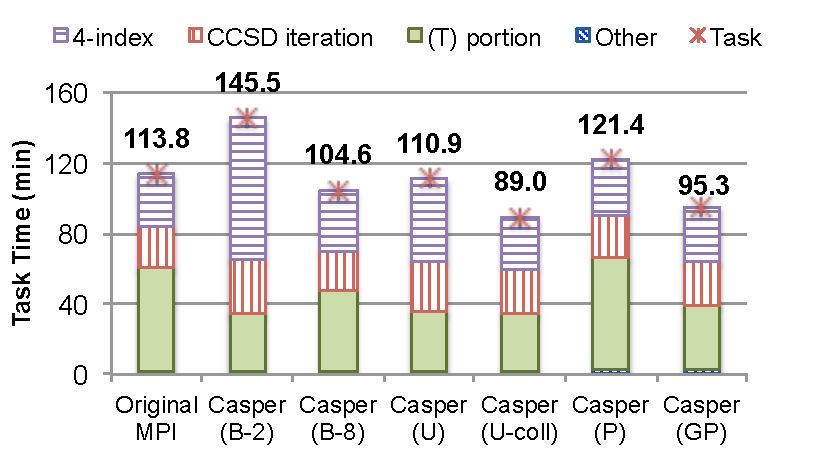
\includegraphics[width=0.64\columnwidth]{figures/adpt-casper/eva_edision_nw_tet_ccsd_t_n240_adpt.pdf}
  \label{fig:eva-edison-nw-ccsdt-tet-adpt}
}
\subfigure[4-Index Profiling]{
  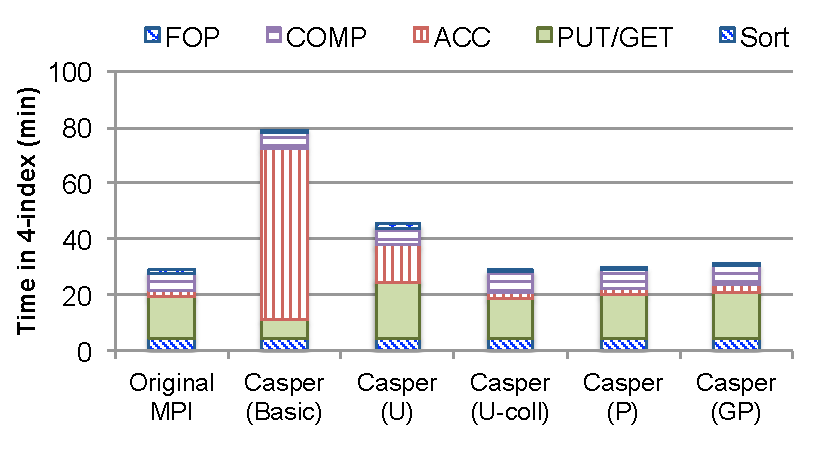
\includegraphics[width=0.64\columnwidth]{figures/adpt-casper/eva_edision_nw_tet_ccsd_t_n240_adpt_4idx.pdf}
  \label{fig:eva-edison-nw-ccsdt-tet-adpt-4idx}
}
% \subfigure[CCSD iteration]{
%   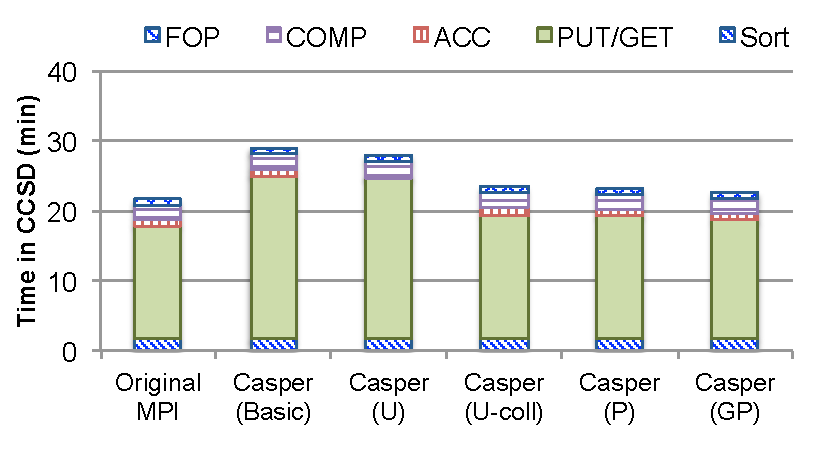
\includegraphics[width=0.64\columnwidth]{figures/adpt-casper/eva_edision_nw_tet_ccsd_t_n240_adpt_ccsd.pdf}
%   \label{fig:eva-edison-nw-ccsdt-tet-ccsd-da}
% }
\subfigure[(T) portion Profiling]{
  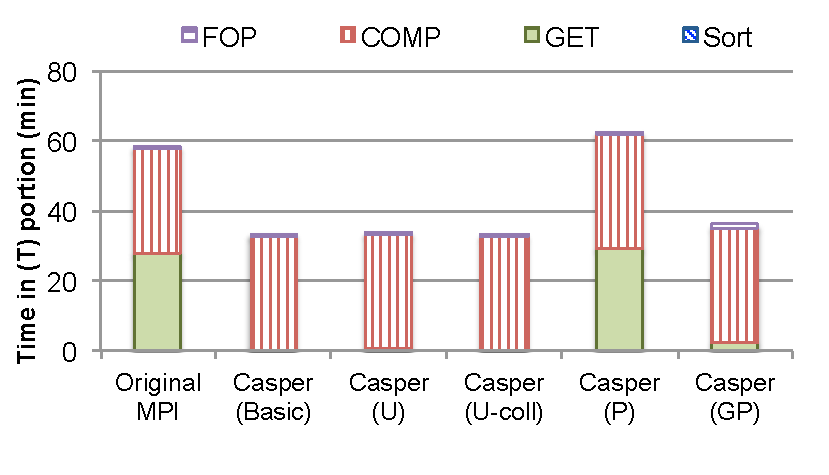
\includegraphics[width=0.64\columnwidth]{figures/adpt-casper/eva_edision_nw_tet_ccsd_t_n240_adpt_t.pdf}
  \label{fig:eva-edison-nw-ccsdt-tet-adpt-t}
}
\caption{Profiling CCSD(T) for Tet-pVDZ problem with Casper adaptation on 240 cores.}
\label{fig:eva-nwchem-acenes-adpt}
\end{figure*}

As shown in Figure~\ref{fig:eva-edison-nw-ccsdt-tet-adpt-4idx},
the \libname(U) approach can reduce the overhead of ACCUMULATE communication
in 4-index phase since it disables the asynchronous progress at window
allocation time, however, the overhead is still higher that the cost in
original MPI because it does not adapt for existing windows thus over
workload issue still exists on those existing windows and consequently
degrade the performance of ACCUMULATE.
The \libname(U-coll), \libname(P) and \libname(GP)approaches completely
resolve such performance degradation, this is because
both approaches allow asynchronous progress to be changed at both
window allocation time for new windows, and at Ga\_sync time for all
existing windows.
On the other hand, we also notice that, all the adaptation approaches shows
similar performance in the PUT/GET part as that in original MPI, which is
worse than the basic Casper. This is because asynchronous progress is
still useful for the PUT/GET part since it performs concurrently with
computation on all processes, however the adaptation approaches entirely
disable asynchronous progress due to large proportion of communication
including both ACCUMULATE and PUT/GET.

For the (T) portion, as shown in
Figure~\ref{fig:eva-edison-nw-ccsdt-tet-adpt-t}, both user-guided
approaches significantly reduce the overhead of GET communication
as that we have provided in basic Casper, however, the \libname(P)
approach cannot achieve the same performance and even shows slightly
performance degradation comparing with the original MPI. This is because,
different from the 4-index and CCSD iteration phases,
the (T) portion is a non-iteration phase consisting of only heavy
computation and enormous GET-flush operations. The window creation
only happens at the start of this phase, and GA\_sync only happens
at the end. \libname(P) still disables asynchronous progress for all
processes at window creation time in this phase, since it is adapted
based on the profiling data got from the previous CCSD iteration
phase, which is communication-intensive. After a short period of
execution, it gets sufficient profiling data to determine the pattern
becomes computation intensive, however, can not get any chance to
re-enable the asynchronous progress till the end of this phase.
Moreover, although \libname(P) disables asynchronous progress,
the cores dedicated to ghost processes still could not be reused in
user computation, thus it shows slightly performance degradation even
comparing with the original MPI.

The \libname(GP) approach overcomes the above issue, it reduces
most overhead of the GET communication but is still slightly worse than
that in basic Casper and the user-guided approaches. This
is because, each user process does not update its local status
collectively, thus it takes several rounds of background ghost
synchronization to globally enable the asynchronous progress on
all user processes.

\subsubsection{Ghost Synchronization Interval}
As we have discussed in Figure~\ref{fig:eva-edison-nw-ccsdt-tet-adpt},
the ghost-assisted \libname(GP) approach even improves the self-profiling
based adaptation, especially overcomes the issue in the (T) portion phase.
However, this approach requires user specified interval for the background
synchronization among ghost processes, insufficient synchronization times
may delay the change of asynchronous progress, but too frequent synchronization
may cause additional communication overhead. The optimal value can vary
on different platform and for different computation problems. In this paper,
we manually compare the task execution time with 1, 2, 4 and 6 minutes
as the interval of background synchronization as shown in
Figure~\ref{fig:eva-nwchem-acenes-tet-gadpt}. The best performance is
delivered when setting interval to 4 minutes on our platform. The
4-index phase and (T) portion phase show different trend with increasing
interval time. As shown in Figure~\ref{fig:eva-edison-nw-ccsdt-tet-gadpt-4idx},
heavy overhead has been observed in the ACCUMULATE communication with
1 and 2 minutes interval time because too frequent synchronization,
such overhead is significantly reduced after reducing the frequency
of synchronization by increasing the interval time.
Figure~\ref{fig:eva-edison-nw-ccsdt-tet-gadpt-t} shows different trend
for the (T) portion phase. The GET communication benefits from smaller
interval time, because it highly replies on the asynchronous progress
and frequent synchronization can enable the asynchronous progress earlier.


\begin{figure*}
\centering
\subfigure[Task execution time]{
  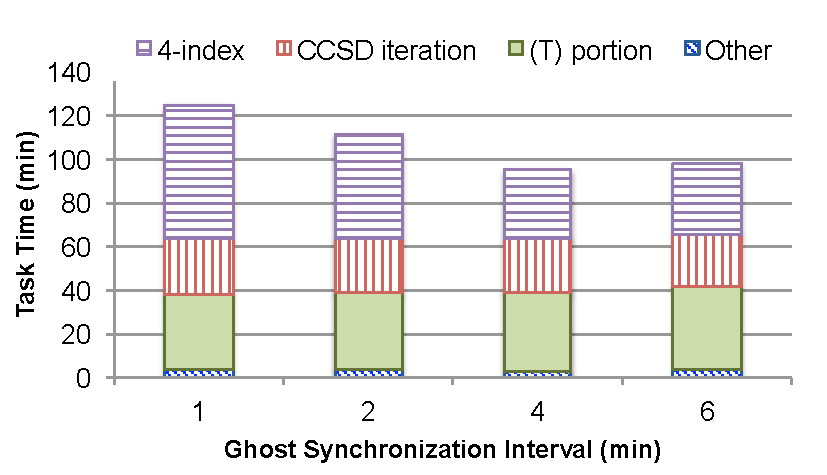
\includegraphics[width=0.64\columnwidth]{figures/adpt-casper/eva_edision_nw_tet_ccsd_t_n240_gadpt.pdf}
  \label{fig:eva-edison-nw-ccsdt-tet-gadpt}
}
\subfigure[4-index profiling]{
  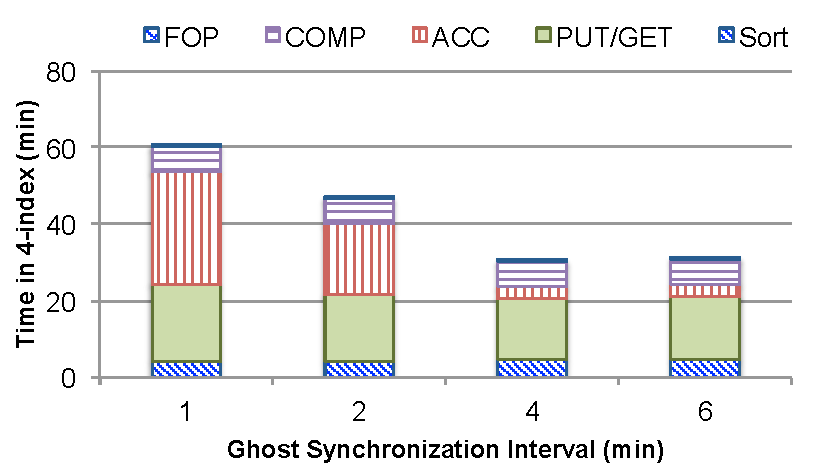
\includegraphics[width=0.64\columnwidth]{figures/adpt-casper/eva_edision_nw_tet_ccsd_t_n240_gadpt_4idx.pdf}
  \label{fig:eva-edison-nw-ccsdt-tet-gadpt-4idx}
}
\subfigure[(T) portion profiling]{
  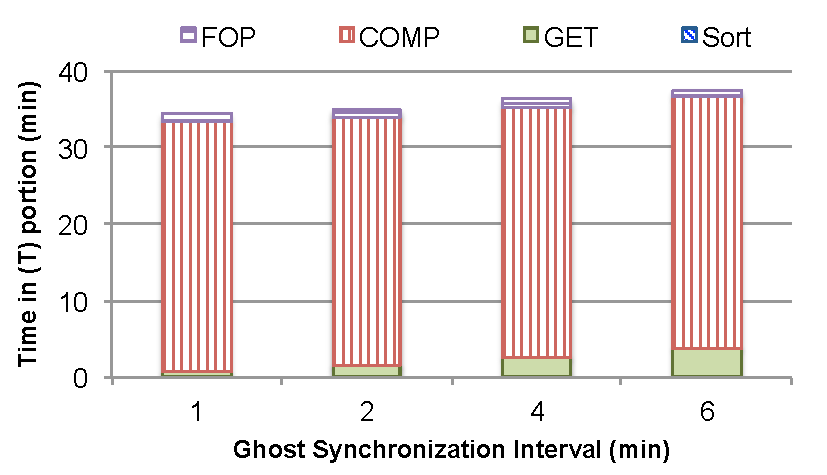
\includegraphics[width=0.64\columnwidth]{figures/adpt-casper/eva_edision_nw_tet_ccsd_t_n240_gadpt_t.pdf}
  \label{fig:eva-edison-nw-ccsdt-tet-gadpt-t}
}
\caption{CCSD(T) for Tet-pVDZ on 240 cores with \libname(GP) adaptation using varying synchronization interval.}
\label{fig:eva-nwchem-acenes-tet-gadpt}
\end{figure*}